\section{Dense neural networks}

\subsection{}

\begin{frame}
    \frametitle{The neuron: equations}

    Consider an input $\x \in \Reals^q$.
    \begin{block}{}
        Consider some \emph{weight vector} $\w \in \Reals^q$ and \emph{bias} $b \in \Reals$.
        The mapping
        \begin{align*}
            g &: \Reals^q \to \Reals \\
            &\hspace{1.25ex} \x \mapsto \w \cdot \x + b
        \end{align*}
        is an \alert{affine transformation}.
    \end{block}
    \pause

    Consider a generally nonlinear \alert{activation function} $\sigma: \Reals \to \Reals$.

    \begin{block}{}
        An (artifical) \alert{neuron} is the function $\phi = \sigma \circ g$, i.e.,
        \begin{align*}
            \phi &: \Reals^q \to \Reals \\
            &\hspace{1.25ex} \x \mapsto \sigma(\w \cdot \x + b)
        \end{align*}
    \end{block}
    \pause

    \begin{itemize}
        \item Historically, artificial neuron modeled on biological neurons
        \begin{itemize}
            \item Bio neuron triggers impulse by nonlinear function of inputs
        \end{itemize}
        \item Today, relation is largely only conceptual/philosophical
    \end{itemize}
\end{frame}

\begin{frame}
    \frametitle{The neuron: geometric interpretation}

    \begin{itemize}
        \item Activation functions $\sigma(x)$ typically most ``interesting'' at $x = 0$
        \item For neuron $\phi(x) = \sigma(\w \cdot \x + b)$, \textcolor{Green4}{hyperplane} $\w \cdot \x + b = 0$ is a natural boundary in $\X$
        \item Simple example:
        \begin{itemize}
            \item $\x =$ (sex, age, weight, height, LDL, HDL, exercise hrs/wk, smoker)
            \item $y =$ heart disease risk
            \item Medical intuition: larger risk for men, older, heavier, shorter, higher LDL, lower HDL, less exercise, smoker
            \item Geometric interpretation: draw \textcolor{Green4}{hyperplane} through $\Reals^8$ best separating \alert{high-risk} from \textcolor{blue}{low-risk}
        \end{itemize}
    \end{itemize}

    \centering
    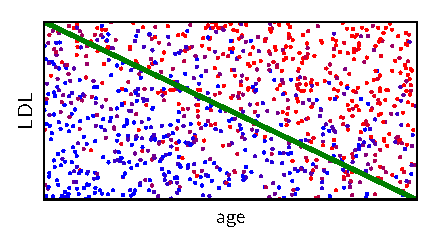
\includegraphics{plane}
\end{frame}

\begin{frame}
    \frametitle{Single hidden-layer neural network: vector equations}

    Consider $n$ neurons each taking in $\x \in \Reals^q$: given
    \begin{itemize}
        \item weight vectors $\w_k \in \Reals^q$, $k = 1, \ldots, n$,
        \item biases $b_k \in \Reals$, $k = 1, \ldots, n$,
    \end{itemize}
    \begin{block}{Hidden layer}
        \vspace{-1em}
        \begin{align*}
            z_k &= \sigma(\w_k \cdot \x + b_k), \quad k = 1, \ldots, n \\
            \z &= \begin{bmatrix} z_1 & \cdots & z_n \end{bmatrix} \in \Reals^n
        \end{align*}
    \end{block}
    \pause

    Let the model output $\y \in \Reals^p$ be affine transformations of $\z$: given
    \begin{itemize}
        \item weight vectors $\v_k \in \Reals^n$, $k = 1, \ldots, p$
        \item biases $c_k \in \Reals$, $k = 1, \ldots, p$
    \end{itemize}
    \begin{block}{Single hidden-layer neural network}
        \vspace{-1em}
        \begin{align*}
            y_k &= \v_k \cdot \z + c_k, \quad k = 1, \ldots, p \\
            \y &= \begin{bmatrix} y_1 & \cdots & y_p \end{bmatrix}
        \end{align*}
    \end{block}
\end{frame}

\begin{frame}
    \frametitle{Single hidden-layer neural network: figure}

    \centering
    \begin{tikzpicture}[>=latex, node distance=9mm]
    % Inputs.
    \uncover<+->{
        \node (x1) [scalar] {$x_1$};
        \node (x2) [scalar, right=of x1] {$x_2$};
        \node (x3) [scalar, right=of x2] {$\cdots$};
        \node (x4) [scalar, right=of x3] {$x_q$};

        \node [right=1.25cm of x4] {$\x$};

    }

    \uncover<+->{
        % Hidden layer.
        \draw [very thick, rounded corners, fill=red!10]
        (-1.2, 0.9) rectangle (6.27, 3.5);

        % Hidden layer combinations.
        \node (affine x1) [affine, above=of x1, xshift=-5mm] {affine};
        \node (affine x2) [affine, right=6mm of affine x1] {affine};
        \node (affine x3) [affine, right=6mm of affine x2] {affine};
        \node (affine x4) [affine, right=6mm of affine x3] {$\cdots$};
        \node (affine x5) [affine, right=6mm of affine x4] {affine};

        \node [right=4.3mm of affine x5] {$\w_k \cdot \x + b_k$};
    }

    \uncover<+->{
        % Hidden layer activations.
        \foreach \i in {1, 2, 3, 5} {
            \node (sigma\i) [activation, above=4mm of affine x\i] {$\sigma$};
        }

        \node (sigma4) [activation, above=4mm of affine x4] {$\cdots$};

        \node [right=5.5mm of sigma5] {$z_k = \sigma(\w_k \cdot \x + b_k)$};
    }

    % Output combinations.
    \uncover<+->{
        \node (affine y1) [affine, above=of sigma2] {affine};
        \node (affine y2) [affine, above=of sigma3] {$\cdots$};
        \node (affine y3) [affine, above=of sigma4] {affine};

        \node [right=1.88cm of affine y3] {$y_k = \v_k \cdot \z + c_k$};
    }

    % Outputs.
    \uncover<+->{
        \node (y1) [scalar, above=of affine y1] {$y_1$};
        \node (y2) [scalar, above=of affine y2] {$\cdots$};
        \node (y3) [scalar, above=of affine y3] {$y_p$};

        \node [right=2cm of y3] {$\y$};
    }

    % Connections.

    \foreach \i/\a in {1/130, 2/110, 3/90, 4/70, 5/50} {
        % Inputs to affines.
        \foreach \j/\b in {1/230, 2/257, 3/283, 4/310} {
            \uncover<2->{\draw [path] (x\j.\a) -- (affine x\i.\b);}
        }

        % Hidden layer affines to activations.
        \uncover<3->{\draw [path] (affine x\i) -- (sigma\i);}
    }

    \foreach \j/\b in {1/120, 2/90, 3/60} {
        % Hidden layer activations to output affines.
        \foreach \i/\a in {1/230, 2/250, 3/270, 4/290, 5/310} {
            \uncover<4->{\draw [path] (sigma\i.\b) -- (affine y\j.\a);}
        }

        % Output affines to outputs.
        \uncover<5->{\draw [path] (affine y\j) -- (y\j);}
    }
\end{tikzpicture}

%%% Local Variables:
%%% mode: latex
%%% TeX-master: "../nn"
%%% End:

\end{frame}

\begin{frame}
    \frametitle{Single hidden-layer neural network: matrix equations}

    The equations are more compact in matrix form:
    \begin{itemize}
        \item Weight matrix $\W \in \Reals^{n \times q}$
        \item Bias vector $\b \in \Reals^n$
        \item Element-wise activation function
        \begin{align*}
            \SIGMA &: \Reals^n \to \Reals^n \\
            &\hspace{1.25ex} \begin{bmatrix} \xi_1 & \cdots & \xi_n \end{bmatrix} \mapsto
            \begin{bmatrix} \sigma(\xi_1) & \cdots & \sigma(\xi_n) \end{bmatrix}
        \end{align*}
    \end{itemize}

    \begin{block}{Hidden layer}
        \begin{equation*}
            \z = \SIGMA(\W \x + \b)
        \end{equation*}
    \end{block}
    \pause

    \begin{itemize}
        \item Weight matrix $\V \in \Reals^{q \times n}$
        \item Bias vector $\c \in \Reals^q$
    \end{itemize}

    \begin{block}{Single hidden-layer neural network}
        \begin{equation*}
            \y = \V \z + \c
        \end{equation*}
    \end{block}
\end{frame}

\begin{frame}
    \frametitle{Activation functions}
    \begin{block}{Why do neurons have nonlinear activation functions?}
        If $\sigma$ is linear (including the identity $\sigma(x) = x$, i.e. no activation), the neural network $\f : \x \mapsto \y$ is necessarily linear \\[1ex]
        For $\f$ to be nonlinear, \alert{activation functions must be nonlinear}!
    \end{block}

    In some sense, it doesn't even matter what $\sigma$ is, as long as it's nonlinear. \\[1ex]

    To be more particular, $\sigma$ should
    \begin{itemize}
        \item be fast to compute (will be called gazillions of times)
        \item not lead to vanishing or exploding gradients
    \end{itemize}
\end{frame}

\begin{frame}
    \frametitle{Common activation functions}
    \begin{columns}
        \begin{column}{2.5in}
            \begin{itemize}
                \item \textcolor{Green4}{Standard logistic/sigmoid function: $\sigma(x) = \dfrac{1}{1 + e^{-x}} = \dfrac{\tanh(x) + 1}{2}$}
                \begin{itemize}
                    \item Used to be preferred
                    \item Now thought to be too slow
                    \item Suffers from vanishing gradients
                \end{itemize}
                \item \textcolor{blue}{Rectified linear unit (ReLU): $\sigma(x) = \max(0, x)$}
                \begin{itemize}
                    \item Most common, but suffers from vanishing gradients
                \end{itemize}
                \item \textcolor{red}{Leaky/parametric ReLU} \citep{MaasICML13}:
                \textcolor{red}{
                    $\sigma(x) = \begin{cases}
                        x &\mid x \ge 0 \\
                        \alpha x &| x < 0
                    \end{cases}$
                }
                \item \textcolor{Magenta3}{Exponential linear unit (ELU)} \citep{ClevertICLR16}:
                \textcolor{Magenta3}{
                    $\sigma(x) = \begin{cases}
                        x &\mid x > 0 \\
                        \alpha (e^x - 1) &\mid x \le 0
                    \end{cases}$
                }
            \end{itemize}
        \end{column}
        \begin{column}{2in}
            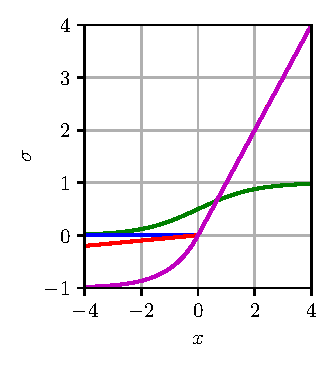
\includegraphics{activations}
        \end{column}
    \end{columns}
\end{frame}

\begin{frame}
    \frametitle{Deep neural networks}

    No reason to stop at only one hidden layer!

    \vspace{1mm}
    \begin{tikzpicture}[node distance=6mm]
    % Layer 1.
    \uncover<2->{\node (n11) [neuron] {};}

    \foreach \i in {1, ..., 4} {
        \pgfmathtruncatemacro{\j}{\i + 1}
        \uncover<2->{\node (n1\j) [neuron, right=of n1\i] {};}

        % Inputs.
        \node (x\i) [io, below=of n1\i, xshift=6mm] {};
        % Layer 2.
        \uncover<3->{\node (n2\i) [neuron, above=of n1\i, xshift=6mm] {};}
    }

    \foreach \i in {1, ..., 3} {
        % Invisible layer 3.
        \node (n3\i) [minimum width=5mm, above=of n2\i, xshift=5mm] {};
        % Invisible layer 4.
        \node (n4\i) [above=4mm of n3\i] {};
    }

    % Etc.
    \uncover<4->{\node (etc) [above=8mm of n22, xshift=6mm] {$\vdots$};}

    \uncover<5->{
        \node (nl1) [neuron, above=of etc, xshift=-6mm] {};
        \node (nl2) [neuron, right=of nl1] {};
    }

    % Outputs.
    \uncover<6->{
        \node (y2) [io, above=of nl1] {};
        \node (y3) [io, above=of nl2] {};
        \node (y1) [io, left=of y2] {};
        \node (y4) [io, right=of y3] {};
    }

    \node [right=of x4, xshift=5.5mm] {$\x \in \Reals^q$};
    \uncover<2->{
        \node [right=of n15] {$\z_1 = \SIGMA(\W_1 \x + \b_1) \in \Reals^{n_1}$};
    }
    \uncover<3->{
        \node [right=of n24, xshift=5.4mm] {$\z_2 = \SIGMA(\W_2 \z_1 + \b_2) \in \Reals^{n_2}$};
    }
    \uncover<4->{
        \node [right=of n33, yshift=-2mm, xshift=1.64cm] {$\vdots$};
        \node [right=of etc, yshift=-1mm, xshift=2.28cm] {$\z_i = \SIGMA(\W_i \z_{i-1} + \b_i) \in \Reals^{n_i}$};
    }
    \uncover<5->{
        \node [right=of n43, yshift=5mm, xshift=1.76cm] {$\vdots$};
        \node [right=of nl2, xshift=1.68cm] {$\z_l = \SIGMA(\W_l \z_{l-1} + \b_l) \in \Reals^{n_l}$};
    }
    \uncover<6->{\node [right=of y4, xshift=5.4mm] {$\y = \V \z_l + \cc \in \Reals^p$};}

    \foreach \i in {1, ..., 4} {
        \foreach \j in {1, ..., 5} {
            \uncover<2->{\draw [path] (x\i.90) -- (n1\j.270);}
            \uncover<3->{\draw [path] (n1\j.90) -- (n2\i.270);}
        }

        \foreach \j in {1, ..., 3} {
            \uncover<4->{\draw [path] (n2\i.90) -- (n3\j.270);}
        }
    }

    \foreach \i in {1, 2} {
        \foreach \j in {1, ..., 3} {
            \uncover<5->{\draw [path] (n4\j.90) -- (nl\i.270);}
        }

        \foreach \j in {1, ..., 4} {
            \uncover<6->{\draw [path] (nl\i.90) -- (y\j.270);}
        }
    }
\end{tikzpicture}

%%% Local Variables:
%%% mode: latex
%%% TeX-master: "../nn"
%%% End:

    \vspace{1mm}

    Common but not necessary for $\SIGMA$ to be the same in each layer
\end{frame}

\begin{frame}
    \frametitle{Why is deep better than wide?}
    \begin{itemize}
        \item Depth: \# layers
        \item Width: \# neurons in each layer (need not be fixed)
    \end{itemize}
    \pause

    Neural network with $\sigma = \text{ReLU}$ is piecewise linear function
    \begin{itemize}
        \item \alert{Expressivity} of ReLU network measured by \# linear pieces
        \item For a network with width $w$ and depth $l$, \alert{$\max \text{expressivity} \sim w^l$} \citep{Pascanu13,MontufarNIPS14,Chen16}
        \begin{itemize}
            \item Polynomial in width
            \item Exponential in depth!
        \end{itemize}
    \end{itemize}
    \pause

    Common for layers closer to the input to be wider
    \begin{itemize}
        \item Closer to the input $\implies$ more expressive power over output \citep{RaghuICML17}
    \end{itemize}
    \pause

    \begin{block}{}
        Depth is (arguably) the key reason for the ML/AI explosion in the last decade.
        Recall ResNet---152 layers deep!
    \end{block}
\end{frame}

\begin{frame}
    \frametitle{What can dense neural networks model?}
    \begin{block}{Universal approximation theorem}
        Anything, basically, if $\text{width} \to \infty$
        \begin{itemize}
            \item Depth not required; 1 hidden layer is enough
        \end{itemize}
    \end{block}

    Some mild conditions required.
    Limitations on $\sigma$:
    \begin{itemize}
        \item $\sigma$ is sigmoid \citep{CybenkoMCSS89,HornikNN89,HornikNN91}
        \item $\sigma$ can be ReLU, polynomial, Gaussian, etc. \citep{SonodaACHA}
    \end{itemize}
\end{frame}

%%% Local Variables:
%%% mode: latex
%%% TeX-master: "../nn"
%%% End:

